\documentclass[../document.tex]{subfiles}

\begin{document}
	\subsection{Описание проекта}
	\par Система состоит из двух взаимосвязанных частей: API вместе с графическим интерфейсом в виде веб-приложения отвечает за создание, управление и просмотр результатов A/B тестов; исполнитель регулярно проверяет в базе наличие тестов, требующих расчёта результатов, проводит вычисления и записывает результаты в базу данных. Исполнитель и API разворачиваются отдельно, в виде двух контейнеров в составе одного пода Kubernetes\cite{kubernetes}.
	\par Средством реализации системы был выбран язык программирования Python\cite{python}, как наиболее популярный на данный момент язык для обработки данных и библиотека FastAPI\cite{fastapi}. Веб-интерфейс был реализован на языке TypeScript\cite{typescript} с применением фреймворка React\cite{react}.
	\par Статистический тест bootstrap mSPRT выполнен в виде модуля для Python на языке C++ с помощью библиотеки Boost.Python\cite{boost_python} в связи с большими вычислительными затратами и вытекающей из них фактической невозможностью выполнять их на Python.
	\par Для работы с базой данных использовалась ORM Sqlalchemy\cite{sqlalchemy}, работа с данными проводилась с помощью библиотеки pandas. Также использовались различные статистические функции библиотеки statsmodels\cite{statsmodels}.
	\par В качестве базы данных использовалась СУБД MySQL 8.0.16 \cite{mysql}, так как в компании в основном используются именно СУБД MySQL различных версий, и системные администраторы обладают достаточным опытом в администрировании данной СУБД.
	\par Структура системы приведена на рисунках \ref{image:module_plot} и \ref{image:class_plot}.
	\begin{figure}[h]
		\centering
		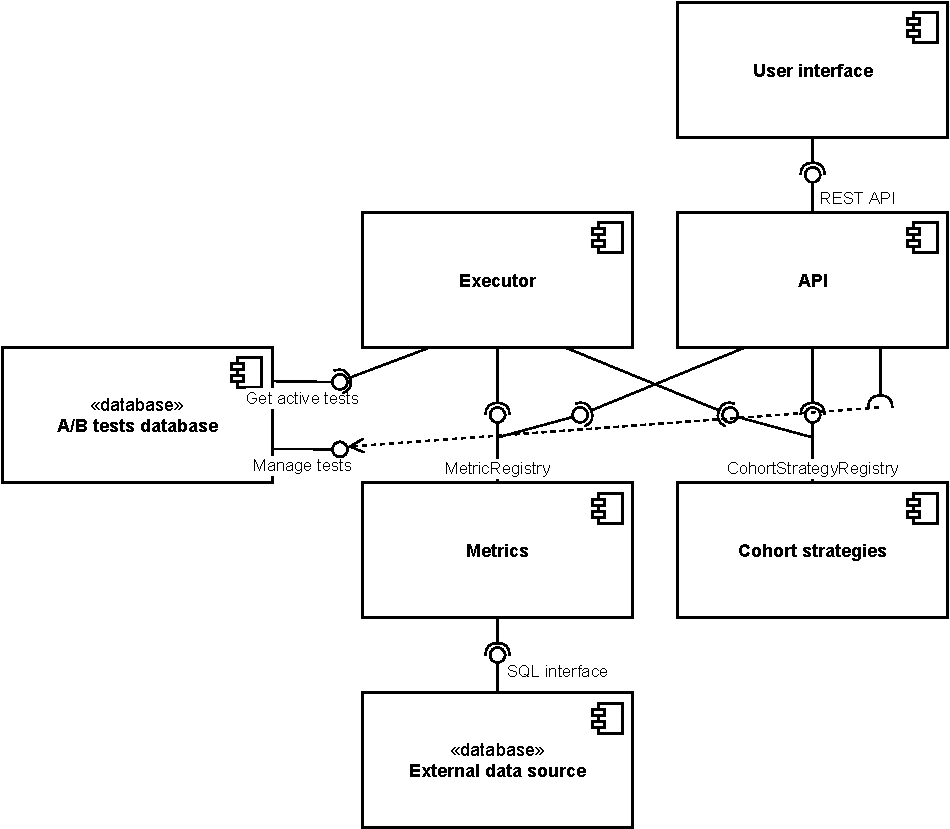
\includegraphics{component_diagram.pdf}
		\caption{\label{image:module_plot}Структура модулей системы}
	\end{figure}
	\begin{figure}[h]
		\centering
		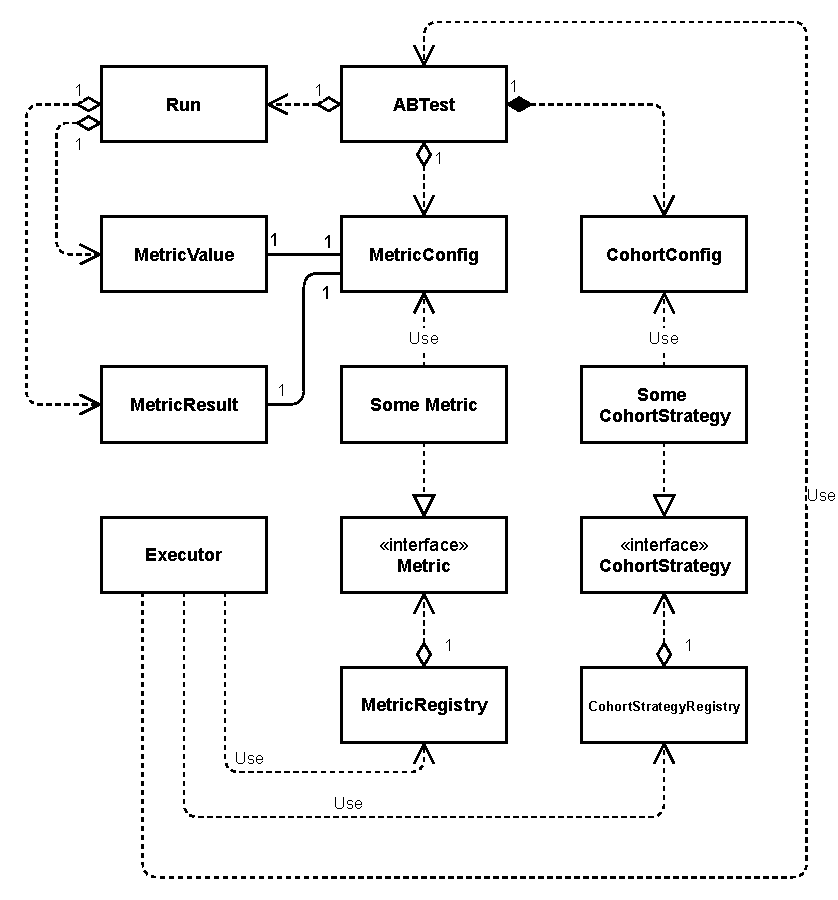
\includegraphics{class_diagram.pdf}
		\caption{\label{image:class_plot}Структура классов системы}
	\end{figure}
	\par Диаграмма состояний теста приведена на рисунке \ref{image:test_state_plot}. В состояние Finished --- тест завершён --- A/B тест может быть переведён как пользователем, вручную, так и по достижению даты окончания теста.
	\begin{figure}[h]
		\centering
		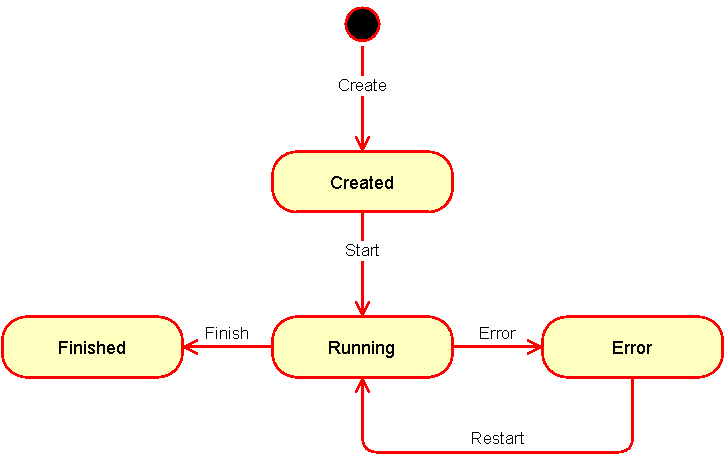
\includegraphics{state_diagram.pdf}
		\caption{\label{image:test_state_plot}Диаграмма состояний A/B теста}
	\end{figure}
	\par Метрики и стратегии распределения по когортам, как самые часто изменяемые элементы системы, были реализованы в виде автоматически регистрирующихся плагинов, регистрация которых происходит во время запуска. Это позволяет добавлять новые метрики и стратегии, не внося изменения в остальную систему.
	\par Также была реализована автоматическая генерация формы создания A/B теста исходя из метаданных плагинов, опять же, для облегчения добавления новых плагинов. Это делается с помощью библиотеки pydantic\cite{pydantic}, генерирующей JSON схему для параметров плагинов, библиотеки react-jsonschema-form, создающей форму по схеме, и доработки генерации схемы для поддержки условных выражений.	
	\FloatBarrier
	\subsection{Реализация и тестирование}
	\subsubsection{Краткие характеристики системы}
	\par Объём работы составил 3300 строк (179 килобайт) на ЯП Python, 300 строк (10 килобайт) --- на C++ и 1200 строк (50 килобайт) --- на Typescript.
	\par Количество модулей составило 10 штук, графический интерфейс содержит 4 страницы.
	\subsubsection{Модули}
	\par Модули кода на Python:
	\begin{enumerate}
		\item \textbf{ab\_testing.api} --- модуль, содержащий реализацию API с применением библиотеки FastAPI. Файл \textbf{ab\_testing.api.api} --- содержит следующие функции:
		\begin{enumerate}
			\item get\_tests (с маршрутом GET /api/v1/tests) --- возвращает список A/B тестов в системе;
			\item get\_test\_by\_id (с маршрутом GET /api/v1/tests/<id>) --- возвращает A/B тест с конкретным id;
			\item create\_new\_test (с маршрутом POST /api/v1/tests) --- создаёт новый A/B тест;
			\item validate\_params --- валидирует параметры A/B теста;
			\item end\_test (c маршрутом POST /api/v1/tests/<id>/end) --- завершает A/B тест;
			\item start\_test (с маршрутом POST /api/v1/tests/<id>/start) --- начинает A/B тест;
			\item retry\_test (с маршрутом POST /api/v1/tests/<id>/retry) --- повторяет попытку посчитать A/B тест;
			\item update\_test (c маршрутом PUT /api/v1/tests/<id>) --- изменяет параметры A/B теста;
			\item test\_schema (с маршрутом GET /api/v1/test\_schema) --- возвращает JSON-схему A/B теста (для формы в графическом интерфейсе);
			\item serve\_app (с маршрутом GET /) --- возвращает веб-приложение на React, являющееся графическим интерфейсом.
		\end{enumerate}
		\item \textbf{ab\_testing.cohorts} --- модуль, содержащий реализацию стратегий распределения пользователей на когорты. Содержит следующие классы:
		\begin{enumerate}
			\item \textbf{CohortStrategy} --- базовый класс стратегии. Определяет методы и поля:
			\begin{enumerate}
				\item name --- внутреннее имя стратегии;
				\item display\_name --- имя, показываемое в интерфейсе;
				\item description --- описание, показываемое в интерфейсе;
				\item parameters\_schema --- pydantic-модель параметров стратегии, используется для валидации;
				\item validate\_parameters --- валидирует параметры стратегии;
				\item get\_cohort --- определяет когорту пользователя;
				\item map\_cohorts --- определяет когорты нескольких пользователей за раз;
				\item n\_cohorts --- возвращает общее количество когорт;
				\item \_\_init\_subclass\_\_ --- при создании нового класса стратегии регистрирует его.
			\end{enumerate}
			\item \textbf{LastDigit} --- стратегия для деления, как правило, пользователей сайта, по последнему символу идентификатора пользователя;
			\item \textbf{RemoteConfig} --- стратегия для деления пользователей мобильного приложения посредством сервиса удалённой конфигурации Google Firebase.
		\end{enumerate}
		\item \textbf{ab\_testing.config} --- содержит утилиты для чтения конфигурации системы из переменных окружения;
		\item \textbf{ab\_testing.database} --- содержит утилиты для взаимодействия с базой данных системы:
		\begin{enumerate}
			\item \textbf{ab\_testing.database.main} --- содержит объявления соединения, а также дополнительную конфигурацию соединения;
			\item \textbf{ab\_testing.database.models} --- содержит модели SQLAlchemy, описывающие таблицы в СУБД MySQL;
			\item \textbf{ab\_testing.database.crud} --- содержит функции для работы с данными в СУБД:
			\begin{enumerate}
				\item get\_active\_tests --- получает из БД список активных A/B тестов;
				\item get\_stopped\_tests --- получает из БД список остановленных A/B тестов;
				\item get\_all\_tests --- получает из БД список всех A/B тестов;
				\item get\_test --- получает из БД A/B тест с нужным id;
				\item get\_last\_successful\_run --- получает из БД последний успешный запуск A/B теста;
				\item create\_test --- создаёт A/B тест в БД;
				\item stop\_test --- останавливает A/B тест;
				\item start\_test --- запускает A/B тест;
				\item retry\_test --- перезапускает A/B тест;
				\item update\_test --- обновляет параметры A/B теста.
			\end{enumerate}
		\end{enumerate}
		\item \textbf{ab\_testing.executor} --- содержит точку входа исполнителя --- модуля, выполняющего расчёт тестов;
		\item \textbf{ab\_testing.metrics} --- содержит реализацию метрик A/B тестов:
		\begin{enumerate}
			\item Класс \textbf{Metric} --- базовый класс метрики. Определяет следующие методы и поля:
			\begin{enumerate}
				\item name --- внутреннее имя метрики;
				\item display\_name --- имя метрики, отображаемое в пользовательском интерфейсе;
				\item description --- описание метрики, отображаемое в пользовательском интерфейсе;
				\item parameters\_schema --- pydantic-модель параметров метрики, используется для валидации;
				\item validate\_parameters --- валидирует параметры метрики;
				\item calculate --- считает значения метрики и статистическую значимость;
				\item \_\_init\_subclass\_\_ --- при создании нового класса метрики регистрирует его.
			\end{enumerate}
			\item calculate\_conversion\_like\_metric --- выполняет расчёт метрики, подобной пользовательской конверсии;
			\item calculate\_ctr\_like\_metric --- выполняет расчёт метрики, подобной CTR, с применением дельта-метода;
			\item calculate\_per\_user\_metric --- выполняет расчёт метрики, формулирующейся как среднее значение некоторого параметра в расчёте на пользователя, с применением bootstrap mSPRT.
		\end{enumerate}
		\par Конкретные метрики представляют собой чувствительную информацию, поэтому их описание не приводится.
		\item \textbf{ab\_testing.schemas} --- содержит pydantic-схемы входных и выходных параметров API;
		\item \textbf{ab\_testing.stats} --- содержит реализации статистических методов, применяемых в системе:
		\begin{enumerate}
			\item mixture\_sprt\_normal --- реализация mSPRT для нормально и биномиально распределённых метрик;
			\item mixture\_sprt\_global\_ctr\_delta\_method --- реализация mSPRT с применением дельта-метода для вычисления \gls{ctr}-подобных метрик;
			\item cuped --- содержит реализацию метода понижения дисперсии CUPED;
			\item catboost --- содержит реализацию метода понижения дисперсии с использованием библиотеки catboost.
		\end{enumerate}
		\item \textbf{ab\_testing.utils} --- содержит прочие функции:
		\begin{enumerate}
			\item window\_funnel --- расчитывает пользовательскую воронку по логам;
			\item get\_complete\_test\_schema --- генерирует JSON схему A/B теста для создания формы в пользовательском интерфейсе.
		\end{enumerate}
	\end{enumerate}
	\par На ЯП C++ в состав системы вошел единственный модуль: \textbf{bootstrap\_msprt}, реализующий статистический критерий bootstrap mSPRT.
	\par На ЯП TypeScript с использованием фреймворка React были реализованы следующие страницы графического интерфейса пользователя.
	\begin{figure}[h]
		\centering
		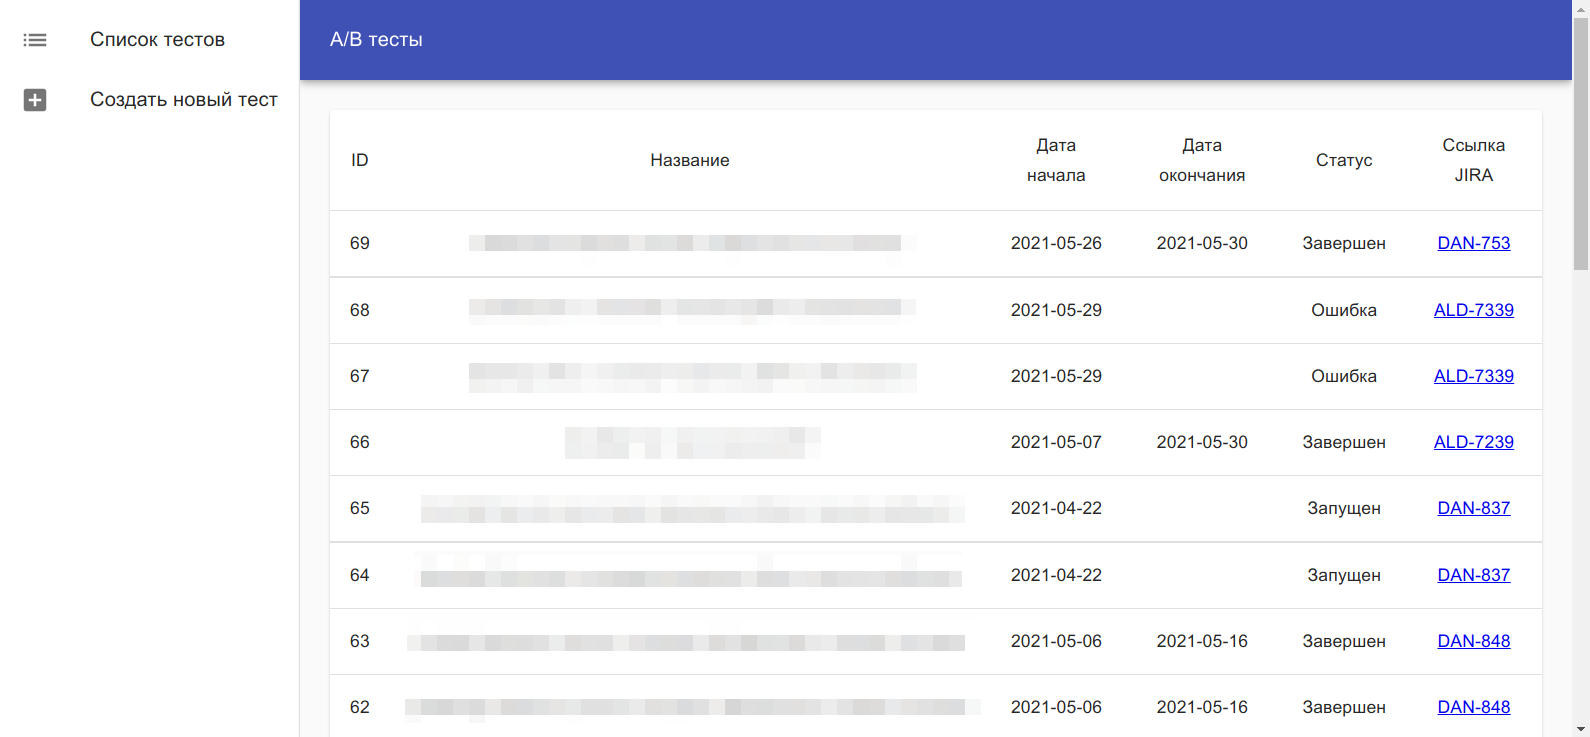
\includegraphics[width=\linewidth]{main_page.png}
		\caption{\label{image:ab_list}Страница просмотра списка A/B тестов}
	\end{figure}
	\par Страница просмотра списка A/B тестов показана на рисунке \ref{image:ab_list}. Она позволяет просматривать все A/B тесты в системе, их статус и основные параметры.
	\par На рисунке \ref{image:ab_page} показана страница просмотра состояния A/B теста. На этой странице отображаются результаты теста: значения метрик в каждой из когорт и  матрица гипотез, отображающая q-value для каждой пары когорт.
	\par Также эта страница позволяет управлять тестом: запускать, останавливать, перезапускать при ошибке.
	\begin{figure}[h]
		\centering
		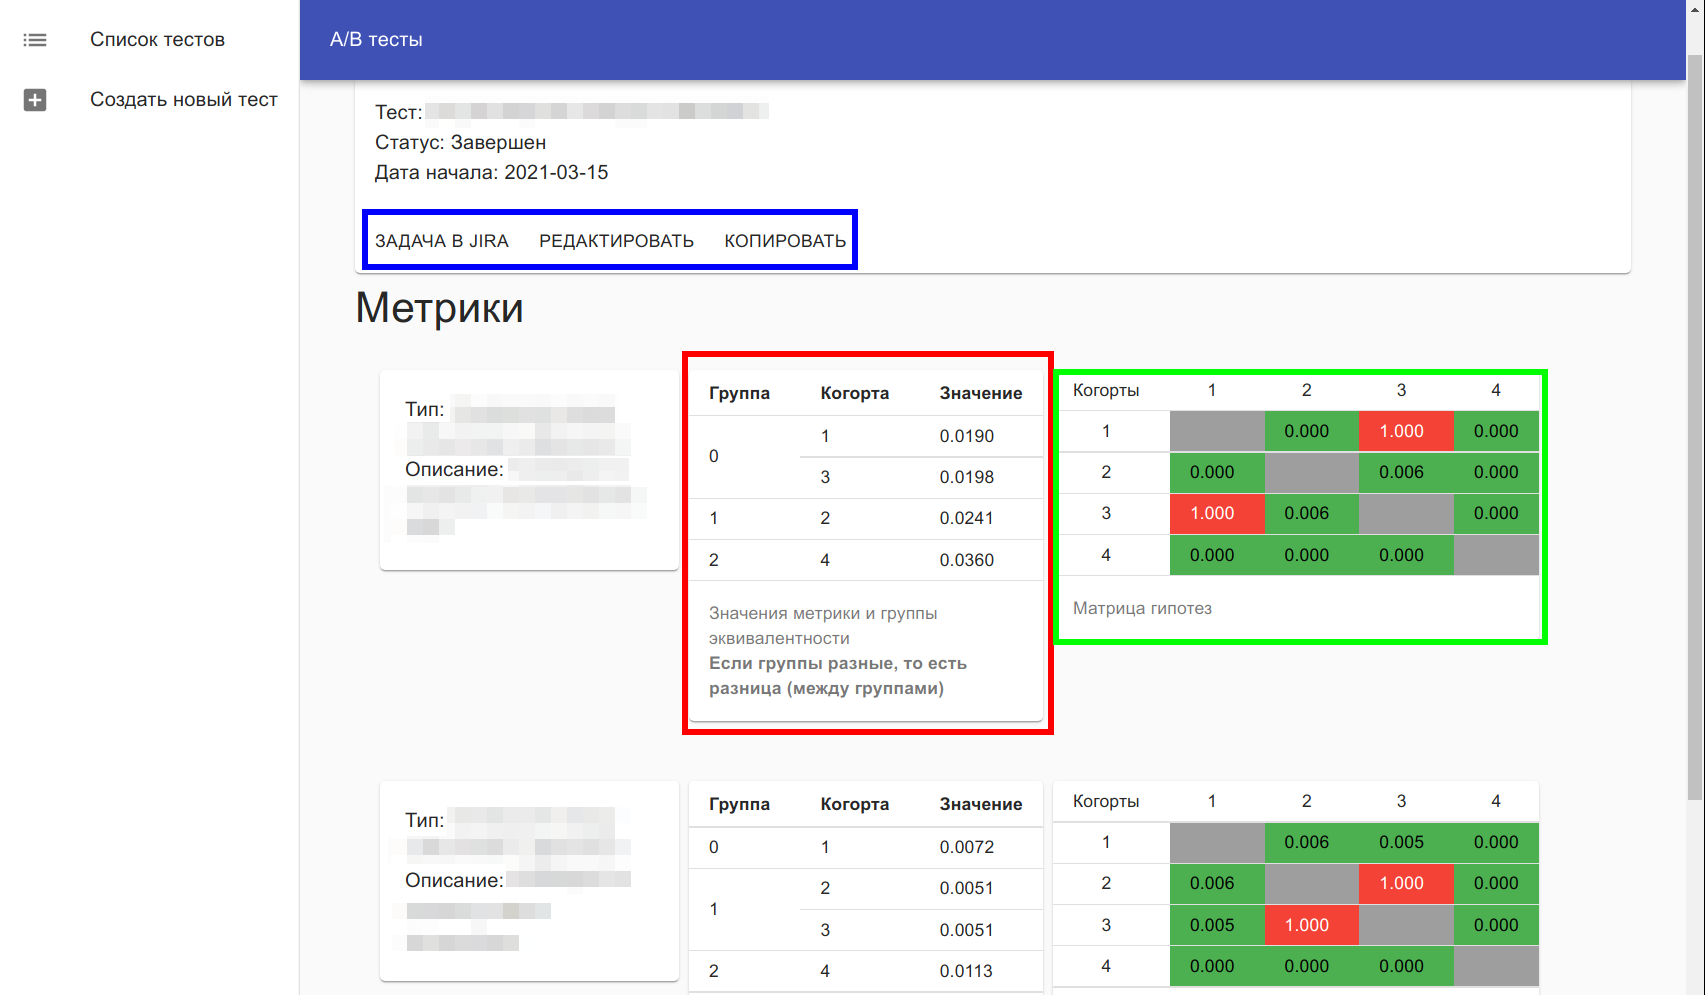
\includegraphics[width=\linewidth]{test_page.png}
		\caption{\label{image:ab_page}Страница просмотра состояния A/B теста}
	\end{figure}
	\par На рисунке \ref{image:ab_edit} отображена страница редактирования A/B теста (создание теста происходит через эту же форму). На странице заполняются все параметры теста, распределения по когортам, выбираются метрики теста и заполняются их параметры.
	\begin{figure}[h]
		\centering
		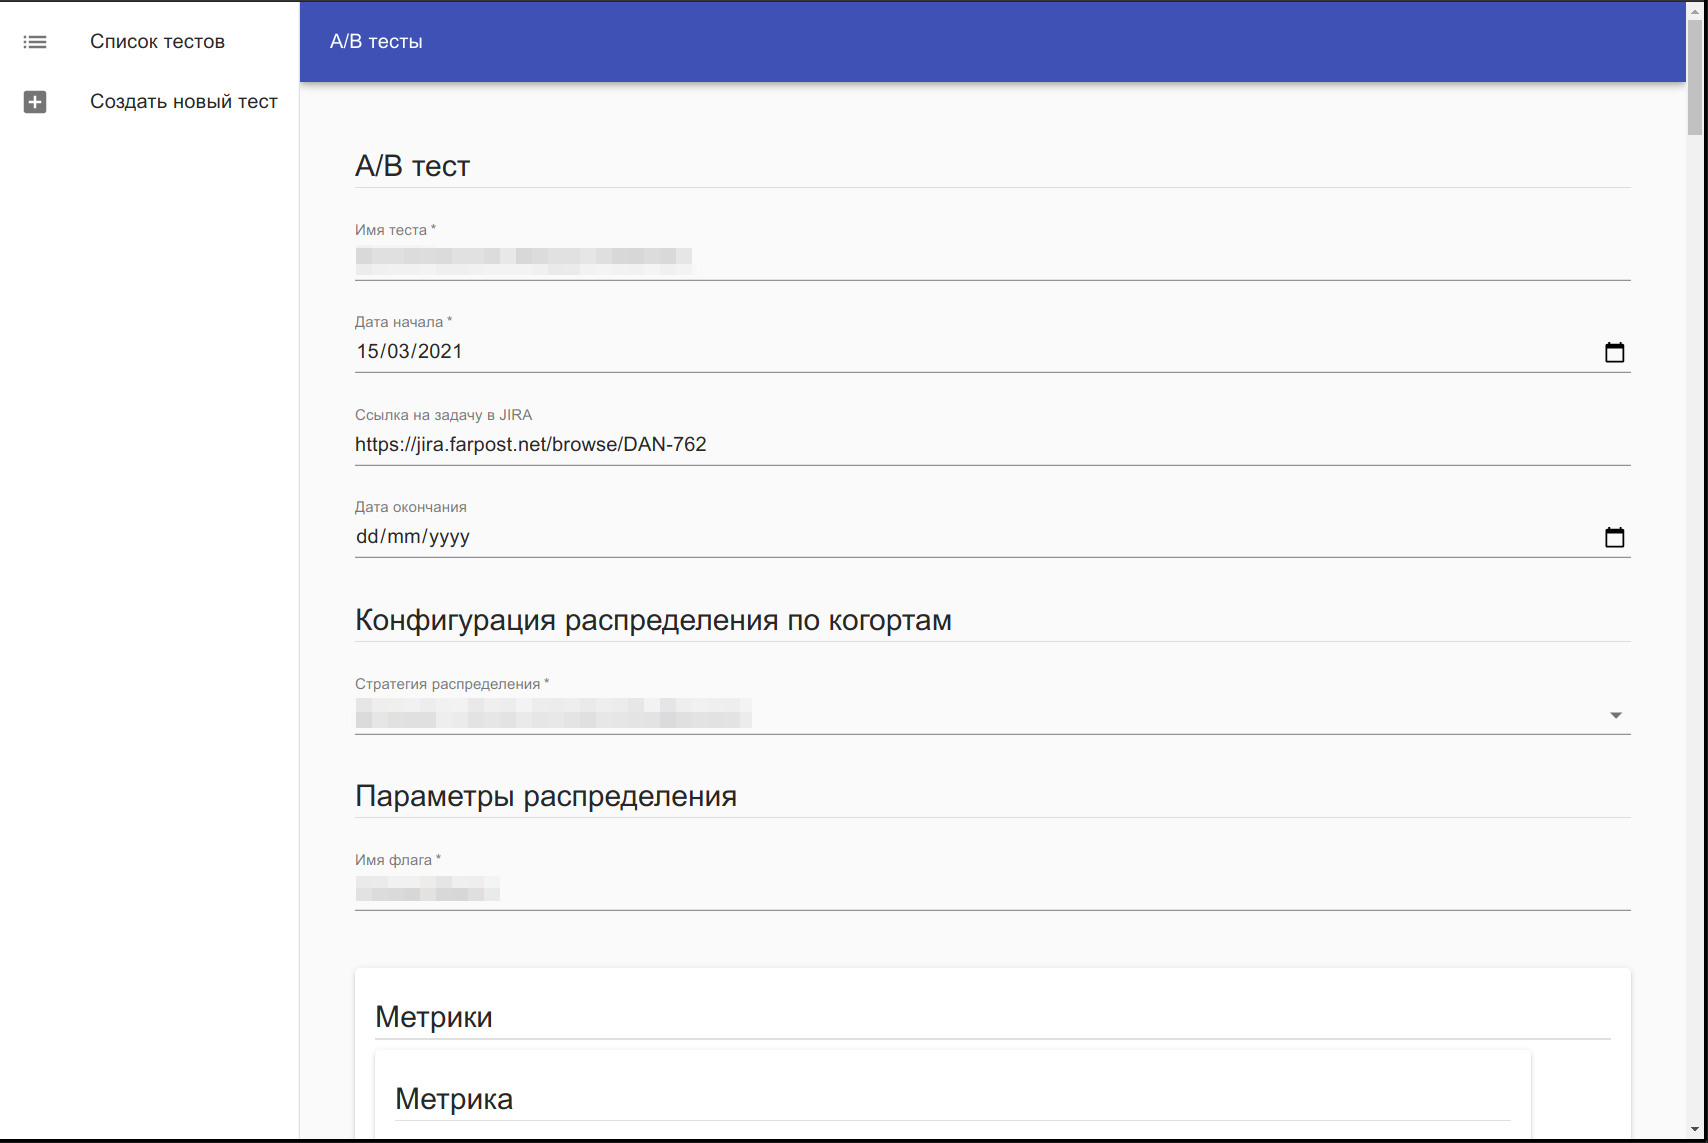
\includegraphics[width=\linewidth]{edit_page.png}
		\caption{\label{image:ab_edit}Страница редактирования A/B теста}
	\end{figure}
	\FloatBarrier
	\subsubsection{Проблемы при реализации}
	\par Первой проблемой при реализации стала недостаточная производительность интерпретатора ЯП Python. При попытке реализовать на нём bootstrap mSPRT вычисление в среднем занимало 12 часов, что было непреемлемо даже для небольшого количества A/B тестов.
	\par Было предпринято несколько попыток решения данной проблемы. Первым вариантом стало использование numba --- JIT компилятора для подмножества Python, в основном связанном с библиотекой numpy. Это позволило ускорить вычисления примерно в 12 раз, до одного часа на запуск статистического критерия, но побочным эффектом стал повышенный расход памяти, из-за необходимости реализовать все операции с применением функций numpy.
	\par В связи с неудовлетворительными характеристиками было принято решение реализовать bootstrap mSPRT в виде расширения для ЯП Python на ЯП C++, используя для этого библиотеки Boost.Python и Boost.Numpy. Используя варианты std::transform из версии языка C++17, удалось получить лаконичное решение, которое позволило ускорить вычисления ещё в 6 раз, до 10 минут на запуск критерия. Именно это решение используется в итоговом варианте системы.
	\par Большой проблемой стало отсутствие на <<Дроме>> устоявшейся системы аналитики и неоднородность существующей инфраструктуры. Это приводит к тому, что метрики могут иметь разную структуру и сильно отличаться в плане механизма подсчёта друг от друга. Более того, такая же проблема существует и в разделении пользователей на когорты.
	\par Чтобы упростить добавление новых метрик и стратегий разделения пользователей, необходимо было сделать эти части системы модульными. Это было реализовано через саморегистрирующиеся классы. Данное решение позволило добавлять новые классы, не внося изменений в другие файлы.
	\par Следующей важной проблемой стала реализация графического интерфейса создания теста в условиях большого разнообразия метрик. Необходимость доработки интерфейса для каждой новой метрики свела бы на нет всю модульность системы.
	\par Таким образом, появилась задача автоматической генерации формы создания теста. Библиотека pydantic уже поддерживала генерацию JSON схемы по модели на Python, и эти модели уже использовались как для описания API, так и для валидации параметров стратегий разделения на когорты и метрик.
	\par С другой стороны, для React была обнаружена библиотека react-jsonschema-form, которая обладала возможностью создавать формы для введения данных по JSON схеме. Также библиотека поддерживала условные выражения в JSON схеме, что является нестандартным расширением.
	\par Для реализации добавления теста через форму была реализована функция, которая дополняла JSON схему теста схемами конфигураций метрик и стратегий распределения пользователей, таким образом, что параметры метрики показывались только при выборе этой метрики в интерфейсе, аналогичным образом --- для стратегий распределения пользователей.
	\par Данное решение позволяет вносить изменения в код системы, и, в частности, добавлять новые метрики, не внося изменений в код графического интерфейса.
	\par Также, необходимо было придумать способ отображения результатов теста в интерфейсе. Если бы все тесты проводились только на 2 когортах, то это не было бы значительной проблемой: есть только 2 исхода: различия либо статистически значимы, либо незначимы.
	\par Когда вариантов становится больше, могут возникнуть различные ситуации, например, что группа когорт без различий между собой может иметь статистически значимые различия с другой группой когорт.
	\par Одним из вариантов решения подобной задачи является применение процедур нахождения лучшего варианта в статистической постановке, как, например, в работе \cite{sequential_choosing_best}. Однако, такой вариант не всегда подходит для разрабатываемой системы: часто A/B тесты проводятся не для того, чтобы выявить улучшение метрики, а чтобы не допустить её ухудшения.
	\par В итоге был реализован следующий вариант: когорты сравниваются попарно, с поправкой Беньямини-Гохберга \cite{benjamini_hochberg}. После этого мы получаем некоторый граф, вершинами которого являются когорты, компоненты связности которого описывают группы эквивалентности этих когорт.
	\par При отображении когорты группируются и выводятся вместе с значениями метрик в них. Дополнительно выводится матрица значений q-value для каждой пары когорт для дополнительной информации о структуре этого графа.
	\par Данное решение обладает тем недостатком, что возможна ситуация, в которой, например, при наличии 3 когорт: А, Б и В, когорты А и Б, Б и В не будут иметь статистически значимые различия, а когорты А и В --- будут. Тогда алгоритм объединит все 3 когорты в одну группу эквивалентности.
	\par Альтернативным правильным решением было бы применение некого статистического метода, сочетающего ранжирование и множественное тестирование гипотез, однако, на момент написания данной работы такого или подобного метода обнаружить не удалось.
	\subsection{Практическое применение и внедрение}
	\par Внедрение системы началось ещё на этапе прототипирования --- когда система не имела даже веб-интерфейса. Изначально она использовалась больше для апробации самой идеи автоматизированного A/B тестирования, нежели для проведения тестов.
	\par Полноценное внедрение было осуществлено с внедрением графического интерфейса. Изначально графический интерфейс не позволял создавать A/B тест, и создание производилось вручную, через JSON API. Однако даже возможность наблюдать за результатами теста в приближенном к реальному времени произвела положительное впечатление на основных пользователей --- менеджеров продуктов.
	\par Внедрение постепенно происходило по мере разработки как самой системы, так и пользовательского интерфейса. На текущий момент система позволяет менеджерам самостоятельно создавать A/B тесты, и, таким образом, проводить тесты без участия аналитиков данных.
	\par За полгода эксплуатации системы через неё было полностью проведено 68 A/B тестов, что позволило сэкономить около 550 часов работы аналитиков, согласно учёту времени в таск-трекере JIRA.
\end{document}